\documentclass[border=1pt]{standalone}
\usepackage[dvipsnames]{xcolor}
\usepackage{tikz}                       % Graphen und kommutative Diagramme
\usetikzlibrary{patterns}               % Um schraffierte Formen in der tikzpicture-Umgebung zu zeichnen.
\usetikzlibrary{shapes}                 % Polygone
\newcommand{\ul}[1]{\underline{\smash{#1}}}

\begin{document}
\centering
\begin{minipage}{.4\textwidth}
    \centering
    \resizebox{!}{3.4cm}{
        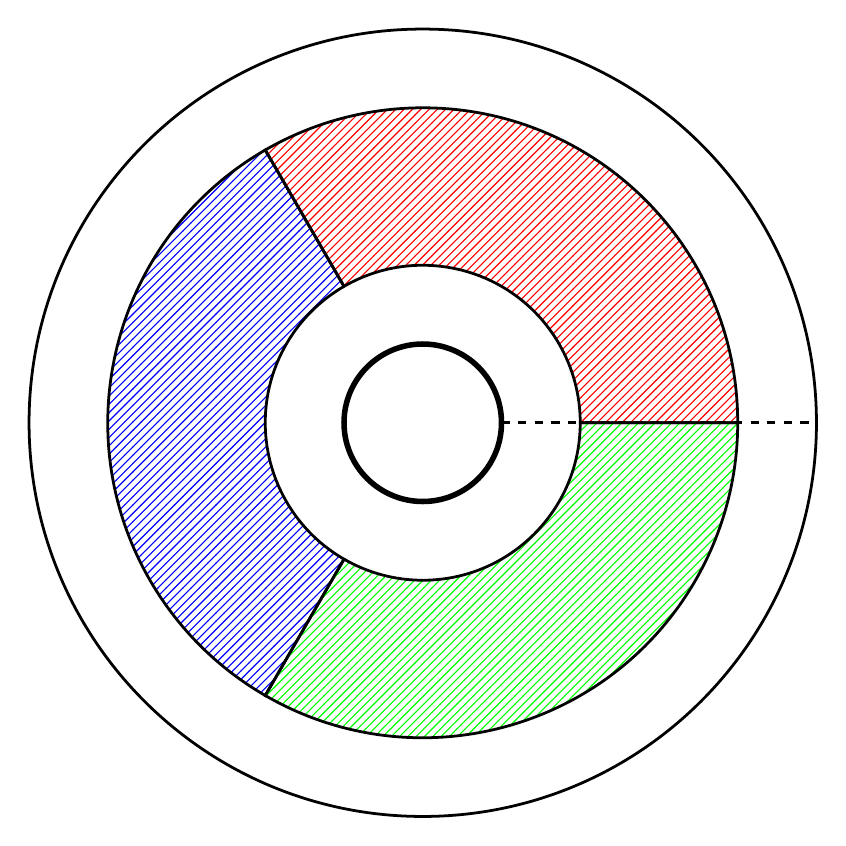
\begin{tikzpicture}[line width=1pt]
            % draw shaded slit box
            \filldraw[pattern=north east lines, pattern color=red] 
            (0 : 2) -- (  0 : 4) arc [radius = 4, start angle =   0, delta angle =  120] 
                    -- (120 : 2) arc [radius = 2, start angle = 120, delta angle = -120] ;
            
            \filldraw[pattern=north east lines, pattern color=blue] 
            (120 : 2) -- (120 : 4) arc [radius = 4, start angle = 120, delta angle =  120] 
                        -- (240 : 2) arc [radius = 2, start angle = 240, delta angle = -120] ;
            
            \filldraw[pattern=north east lines, pattern color=green] 
            (240 : 2) -- (240 : 4) arc [radius = 4, start angle = 240, delta angle =  120] 
                        -- (360 : 2) arc [radius = 2, start angle =   0, delta angle = -120] ;
                    
            % draw inner and outer circles
            \draw[color=black] (0, 0) circle (1);
            \draw[color=black] (0, 0) circle (5);
            
            % draw 0 line
            \draw[color=black, dashed] (0 : 1) -- (0 : 5); 
            
            % draw line width=2pt boundary lines
            \draw[line width=2pt] (0 : 1) arc [radius = 1, start angle = 0, delta angle = 360];  
        \end{tikzpicture}
    }
\end{minipage}
\hspace{1ex}
\begin{minipage}{.4\textwidth}
\centering
\resizebox{!}{4cm}{
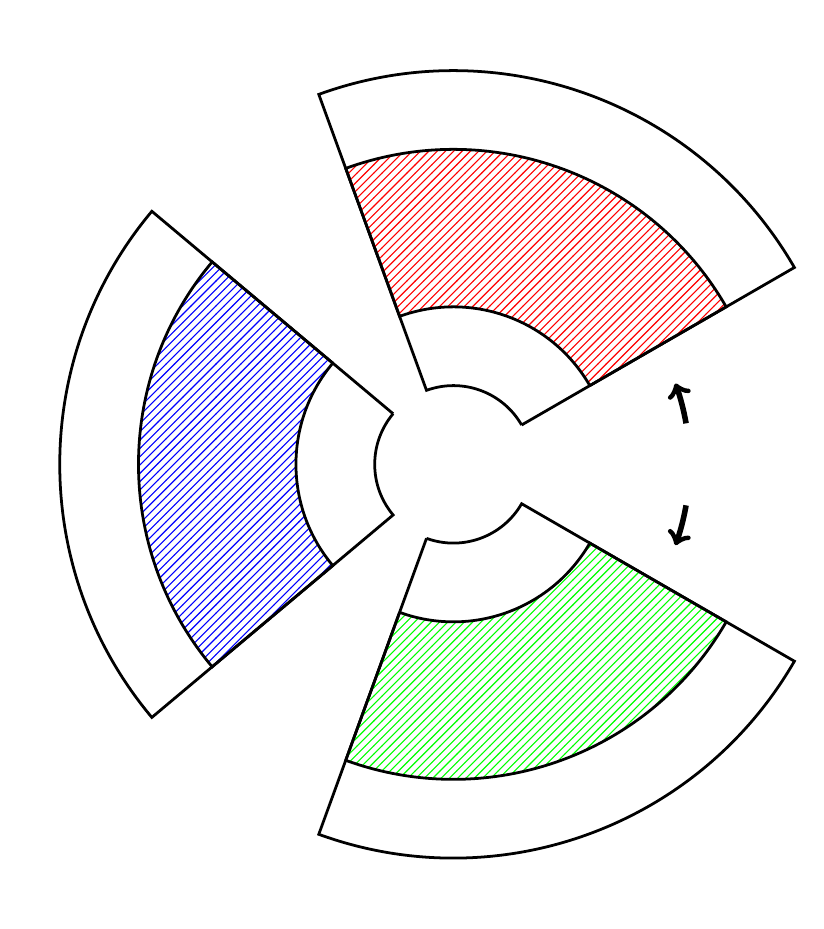
\begin{tikzpicture}[line width=1pt]
    % draw pieces of cake
    \draw (30 : 1) -- (30 : 5)  arc [radius = 5, start angle = 30, delta angle = 80] 
	           -- (110 : 1) arc [radius = 1, start angle = 110, delta angle = -80];
    \draw (140 : 1) -- (140 : 5) arc [radius = 5, start angle = 140, delta angle = 80] 
	           -- (220 : 1) arc [radius = 1, start angle = 220, delta angle = -80];
    \draw (250 : 1) -- (250 : 5)  arc [radius = 5, start angle = 250, delta angle = 80] 
	           -- (330 : 1) arc [radius = 1, start angle = 330, delta angle = -80];
    
    % draw shaded slit box
    \filldraw[pattern=north east lines, pattern color=red] 
      (30 : 2) -- (30 : 4) arc [radius = 4, start angle = 30, delta angle = 80] 
	       -- (110 : 2) arc [radius = 2, start angle = 110, delta angle = -80] ;
    \filldraw[pattern=north east lines, pattern color=blue] 
      (140 : 2) -- (140 : 4) arc [radius = 4, start angle = 140, delta angle = 80] 
	       -- (220 : 2) arc [radius = 2, start angle = 220, delta angle = -80] ;
    \filldraw[pattern=north east lines, pattern color=green] 
      (250 : 2) -- (250 : 4) arc [radius = 4, start angle = 250, delta angle = 80] 
	       -- (330 : 2) arc [radius = 2, start angle = 330, delta angle = -80] ;
     
    % draw arrows
    \draw[<-, line width = 2pt] (20  : 3) arc [radius = 3, start angle = 20, delta angle = -10]; 
    \draw[<-, line width = 2pt] (340 : 3) arc [radius = 3, start angle = 340, delta angle = 10]; 
     
\end{tikzpicture}
}
\end{minipage}

\centering
\begin{minipage}{.4\textwidth}
\centering
\resizebox{!}{5cm}{
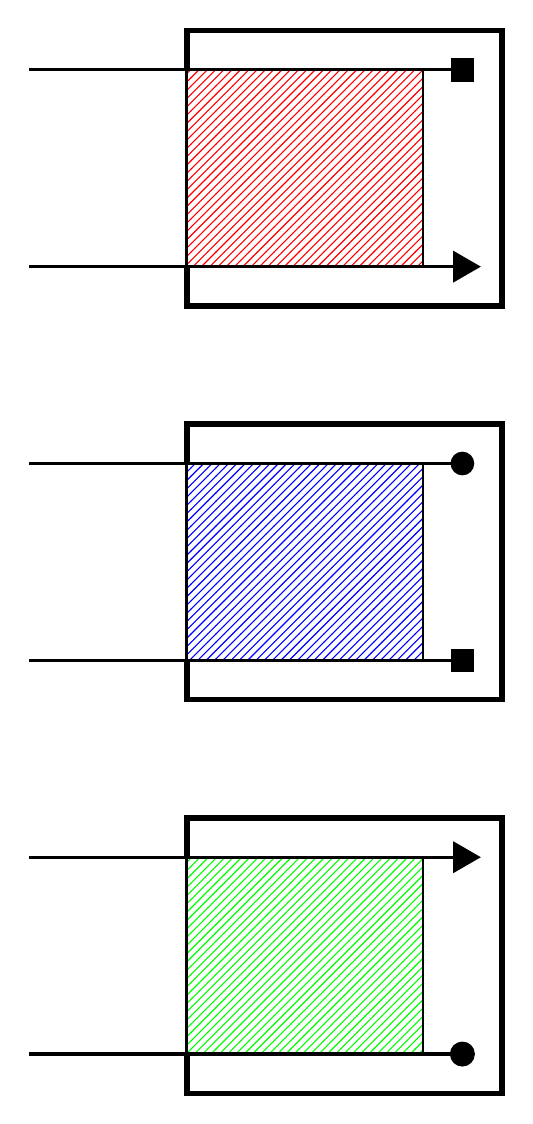
\begin{tikzpicture}[line width=1pt]
% red picture
    % draw outer lines
    \draw (0, 0) -- (4, 0) -- (4, 3.5) -- (0, 3.5) -- (0, 0);
    
    % draw shaded slit box
    \filldraw[pattern=north east lines, pattern color=red] (0, 10.5) -- (3, 10.5) -- (3, 13) -- (0, 13) -- (0, 10.5);
    
    % draw line width=2pt boundary lines
    \draw[line width=2pt] (0, 10.5) -- (0, 10) -- (4, 10) -- (4, 13.5) -- (0, 13.5) -- (0, 13);
    
    % draw slits
    \draw[color=black, line width=1.2pt] (-2, 10.5) -- (3.5, 10.5);
    \draw[color=black, line width=1.2pt] (-2, 13) -- (3.5, 13);
    \node[rotate = 270, scale = 0.6, draw = black, fill = black, regular polygon, regular polygon sides = 3] at (3.5, 10.5) {};
    \node[scale = 0.8, draw = black, fill = black, regular polygon, regular polygon sides = 4] at (3.5, 13) {};
% blue picture
     % draw outer lines
    \draw (0, 5) -- (4, 5) -- (4, 8.5) -- (0, 8.5) -- (0, 5);
    
    % draw shaded slit box
    \filldraw[pattern=north east lines, pattern color=blue] (0, 5.5) -- (3, 5.5) -- (3, 8) -- (0, 8) -- (0, 5.5);
    
    % draw line width=2pt boundary lines
    \draw[line width=2pt] (0, 5.5) -- (0, 5) -- (4, 5) -- (4, 8.5) -- (0, 8.5) -- (0, 8);
    
    % draw slits
    \draw[color=black, line width=1.2pt] (-2, 5.5) -- (3.5, 5.5);
    \draw[color=black, line width=1.2pt] (-2, 8) -- (3.5, 8);
    \node[scale = 0.8, draw = black, fill = black, regular polygon, regular polygon sides = 4] at (3.5, 5.5) {};
    \node[scale = 0.8, draw = black, fill = black, circle] at (3.5, 8) {};
% green picture
    % draw outer lines
    \draw (0, 0) -- (4, 0) -- (4, 3.5) -- (0, 3.5) -- (0, 0);
    
    % draw shaded slit box
    \filldraw[pattern=north east lines, pattern color=green] (0, 0.5) -- (3, 0.5) -- (3, 3) -- (0, 3) -- (0, 0.5);
    
    % draw line width=2pt boundary lines
    \draw[line width=2pt] (0, 0.5) -- (0, 0) -- (4, 0) -- (4, 3.5) -- (0, 3.5) -- (0, 3);
    
    % draw slits
    \draw[color=black, line width=1.2pt] (-2, 0.5) -- (3.5, 0.5);
    \draw[color=black, line width=1.2pt] (-2, 3) -- (3.5, 3);
    \filldraw (3.5, 0.5) circle (4pt);
    \node[rotate = 270, scale = 0.6, draw = black, fill = black, regular polygon, regular polygon sides = 3] at (3.5, 3) {};
\end{tikzpicture}
}
\end{minipage}



\end{document}
